%%%%%%%%%%%%%%%%%%%%%%%%%%%%%%%%%%%%%%%%%%%%%%%%%%%%%%%%%%%%%%%%%%%%%%%%%%%
\subsubsection{\label{sec:Globus-Protocols}Globus Protocols and Terminology}
%%%%%%%%%%%%%%%%%%%%%%%%%%%%%%%%%%%%%%%%%%%%%%%%%%%%%%%%%%%%%%%%%%%%%%%%%%%
The Globus software provides a well-defined set of protocols
that allow authentication, data transfer, and remote job execution.
Authentication is a mechanism by which an identity is verified.
Given proper authentication, authorization to use a resource
is required.
Authorization is a policy that determines who is allowed to do what. 

Condor (and Globus) utilize the following protocols and terminology.
The protocols allow Condor to interact with grid machines toward
the end result of executing jobs.
\begin{description}
\item[GSI]
\index{GSI (Grid Security Infrastructure)}
The Globus Toolkit's Grid Security Infrastructure (GSI) provides essential
\index{Condor-G!GSI}
building blocks for other grid protocols and Condor-G.
This authentication and authorization system
makes it possible to authenticate a user just once,
using public key infrastructure (PKI) mechanisms to verify
a user-supplied grid credential.
GSI then handles the mapping of the grid credential to the
diverse local credentials and authentication/authorization mechanisms that
apply at each site. 
\item[GRAM]
The Grid Resource Allocation and Management (GRAM) protocol supports remote
\index{Condor-G!GRAM}
\index{GRAM (Grid Resource Allocation and Management)}
submission of a computational request (for example, to run a program)
to a remote computational resource,
and it supports subsequent monitoring and control of the computation. 
GRAM is the Globus protocol that Condor-G uses to talk to remote Globus
  jobmanagers.
\item[GASS]
The Globus Toolkit's Global Access to Secondary Storage (GASS) service provides
\index{Condor-G!GASS}
\index{GASS (Global Access to Secondary Storage)}
mechanisms for transferring data to and from a remote HTTP, FTP, or GASS server. 
GASS is used by Condor for the 
\SubmitCmd{gt2} and \SubmitCmd{gt3} \SubmitCmd{grid\_type}s
to transfer a job's files
to and from the machine where the job is submitted and the remote resource.
\item[GridFTP]
GridFTP is an extension of FTP that provides strong security and 
high-performance options for large data transfers.
It is used with the \SubmitCmd{gt4} \SubmitCmd{grid\_type}
to transfer the job's files between the machine where the job
is submitted and the remote resource.
\item[RSL]
RSL is the language GRAM accepts to specify job information.
\item[gatekeeper]
A gatekeeper is a software daemon executing on a remote machine on
the grid.
It is relevant only to the \SubmitCmd{gt2} \SubmitCmd{grid\_type},
and this daemon handles the initial communication between
Condor and a remote resource.
\item[jobmanager]
A jobmanager is
the Globus service that is initiated at a remote resource to submit,
keep track of, and manage grid I/O for jobs running on 
an underlying batch system.
There is a specific jobmanager for each type of
batch system supported by Globus (examples are Condor, LSF, and PBS).

\end{description}


\begin{figure}[hbt]
\centering
\includegraphics{grids/gfig1.eps}
\caption{\label{fig:condorg}Condor-G interaction with Globus-managed resources}
\end{figure}

Figure~\ref{fig:condorg} shows how Condor interacts with Globus software
towards running jobs.
The diagram is specific to the \SubmitCmd{gt2} \SubmitCmd{grid\_type}.
Condor contains a GASS server, used to transfer the executable,
\File{stdin}, \File{stdout}, and \File{stderr} to and from
the remote job execution site.
Condor uses the GRAM protocol to contact the remote gatekeeper
and request that a new jobmanager be started.
The GRAM protocol is also used to when monitoring the job's progress.
Condor detects and intelligently handles cases
such as if the remote resource crashes.

There are now three different versions of the GRAM protocol.
Condor supports all three.
Condor's grid universe uses the \SubmitCmd{grid\_type} command within
a submit description file to distinguish among them.
\begin{description}
\item[gt2]
This initial GRAM protocol is used in Globus Toolkit versions 1 and 2.
It is still used by many production systems.
Where available in the other, more recent versions of the protocol,
\SubmitCmd{gt2} is referred to as the pre-web services GRAM.
\item[gt3]
The \SubmitCmd{gt3} \SubmitCmd{grid\_type} corresponds to
Globus Toolkit version 3 as part of
Globus' shift to web services-based protocols.
It is replaced by  the Globus Toolkit version 4.
An installation of the Globus Toolkit version 3 may also
include the the pre-web services GRAM.
\item[gt4]
The GRAM protocol was introduced in Globus Toolkit version 4 as a more
standards-compliant version of the GT3 web services-based GRAM.
An installation of the Globus Toolkit version 4 may also
include the the pre-web services GRAM.
\end{description}

%%%%%%%%%%%%%%%%%%%%%%%%%%%%%%%%%%%%%%%%%%%%%%%%%%%%%%%%%%%%%%%%%%%%%%%%%%%
\subsubsection{\label{sec:Using-gt2}The gt2 grid\_type}
%%%%%%%%%%%%%%%%%%%%%%%%%%%%%%%%%%%%%%%%%%%%%%%%%%%%%%%%%%%%%%%%%%%%%%%%%%%

\index{universe!globus}
\index{universe!grid, grid\_type gt2}
This section contains what users need to know to 
run and manage jobs under the \SubmitCmd{grid} universe, using the Globus \SubmitCmd{gt2} protocol.
Older submit description files specifying a \SubmitCmd{globus} universe job
will default to this.

\index{Condor-G!job submission}
\index{Condor-G!proxy}
\index{proxy}
Under Condor, successful job submission to the \SubmitCmd{grid} 
\SubmitCmd{universe} with \SubmitCmd{gt2}
requires credentials.
\index{Condor-G!X.509 certificate}
An X.509 certificate is used to create a proxy,
and an account, authorization, or allocation to use a grid resource
is required.
For more information on proxies and certificates,
please consult the Alliance PKI pages at 

\URL{http://archive.ncsa.uiuc.edu/SCD/Alliance/GridSecurity/}

Before submitting a job to Condor under the \SubmitCmd{grid} universe,
use \Prog{grid-proxy-init} to create a proxy.

A job is submitted for execution using the
\Condor{submit} command.
\Condor{submit} takes as an argument
the name of a file called a submit description file.
\index{submit description file!grid universe}
The following example submit description file runs a job on
the Origin2000 at NCSA.

\begin{verbatim}
executable = test
globusscheduler = modi4.ncsa.uiuc.edu/jobmanager
universe = grid
grid_type = gt2
output = test.out
log = test.log
queue
\end{verbatim} 

The 
\SubmitCmd{executable}
for this example is
transferred from the local machine to the remote machine.
By default, Condor transfers the executable, as well as any
files specified by an \SubmitCmd{input} command.
Note that the executable must be compiled for the correct
intended platform.

\index{submit commands!globusscheduler}
The command \SubmitCmd{globusscheduler} is a required command
for Condor-G jobs.
It specifies the scheduling software to be used on the remote resource.
There is a specific jobmanager for each type of
batch system supported by Globus.
The full syntax for this command line appears as
\footnotesize
\begin{verbatim}
globusscheduler = machinename[:port]/jobmanagername[:X.509 distinguished name]
\end{verbatim}
\normalsize
The portions of this syntax specification enclosed within
square brackets (\Lbr and \Rbr) are optional.
On a machine where the jobmanager is listening on a nonstandard port,
include the port number.
The \verb@jobmanagername@
is one of five strings:
\begin{verbatim}
jobmanager
jobmanager-condor
jobmanager-pbs
jobmanager-lsf
jobmanager-sge
\end{verbatim}
The Globus software running on the remote resource
uses the specific string to identify and select the correct service
to perform.
Other \verb@jobmanagername@ strings may be used,
where additional services are defined and implemented.


No input file is specified for this example job.
Any output (file specified by the \AdAttr{output})
or error (file specified by the \AdAttr{error})
is transferred 
from the remote machine to the local machine as it is produced.
This implies that these files may be incomplete in the case
where the executable does not finish running on the remote resource.
The ability to transfer standard output and standard error as
they are produced may be disabled by adding to the submit
description file:
\begin{verbatim}
stream_output = False
stream_error  = False
\end{verbatim}
As a result, standard output and standard error will be transferred
only after the job completes.

The job log file is maintained on the submit machine.

To submit this job to Condor-G for execution on the
remote machine, use
\begin{verbatim}
condor_submit test.submit
\end{verbatim}
where \File{test.submit} is the name of the submit description file.

Example output from 
\Condor{q} for this submission looks like:
\footnotesize
\begin{verbatim}
% condor_q


-- Submitter: wireless48.cs.wisc.edu : <128.105.48.148:33012> : wireless48.cs.wi

 ID      OWNER         SUBMITTED     RUN_TIME ST PRI SIZE CMD
   7.0   epaulson     3/26 14:08   0+00:00:00 I  0   0.0  test

1 jobs; 1 idle, 0 running, 0 held
\end{verbatim}
\normalsize

After a short time, the Globus resource accepts the job.
Again running \Condor{q} will now result in

\footnotesize
\begin{verbatim}
% condor_q


-- Submitter: wireless48.cs.wisc.edu : <128.105.48.148:33012> : wireless48.cs.wi

 ID      OWNER         SUBMITTED     RUN_TIME ST PRI SIZE CMD
   7.0   epaulson     3/26 14:08   0+00:01:15 R  0   0.0  test

1 jobs; 0 idle, 1 running, 0 held
\end{verbatim}
\normalsize

Then, very shortly after that, the queue will be empty again,
because the job has finished:

\footnotesize
\begin{verbatim}
% condor_q


-- Submitter: wireless48.cs.wisc.edu : <128.105.48.148:33012> : wireless48.cs.wi

 ID      OWNER            SUBMITTED     RUN_TIME ST PRI SIZE CMD

0 jobs; 0 idle, 0 running, 0 held
\end{verbatim}
\normalsize


A second example of a submit description file runs the Unix \Prog{ls}
program on a different Globus resource.

\footnotesize
\begin{verbatim}
executable = /bin/ls
Transfer_Executable = false
globusscheduler = vulture.cs.wisc.edu/jobmanager
universe = grid
grid_type = gt2
output = ls-test.out
log = ls-test.log
queue
\end{verbatim} 
\normalsize

In this example, the executable (the binary) has been pre-staged.
The executable is on the remote machine, and it is not to
be transferred before execution.
Note that the required 
\AdAttr{globusscheduler} and \AdAttr{universe}
commands are present.
The command
\begin{verbatim}
Transfer_Executable = false
\end{verbatim}
within the submit description file identifies the executable
as being pre-staged.
In this case, the 
\AdAttr{executable}
command gives the path to the executable on the remote machine.

A third example submits a Perl script to be run as a submitted
Condor job.
The Perl script both lists and sets
environment variables for a job.
Save the following Perl script with the name \File{env-test.pl},
to be used as a Condor job executable.

\begin{verbatim}
#!/usr/bin/env perl

foreach $key (sort keys(%ENV))
{
   print "$key = $ENV{$key}\n"
}

exit 0;
\end{verbatim}

Run the Unix command
\begin{verbatim}
chmod 755 env-test.pl
\end{verbatim}
to make the Perl script executable.

Now create the following submit description file
(Replace \File{biron.cs.wisc.edu/jobmanager} with a resource
you are authorized to use.):

\footnotesize
\begin{verbatim}
executable = env-test.pl
globusscheduler = biron.cs.wisc.edu/jobmanager
universe = grid
grid_type = gt2
environment = foo=bar; zot=qux
output = env-test.out
log = env-test.log
queue
\end{verbatim}
\normalsize

When the job has completed, the output file \File{env-test.out}
should contain something like this:

\footnotesize
\begin{verbatim}
GLOBUS_GRAM_JOB_CONTACT = https://biron.cs.wisc.edu:36213/30905/1020633947/
GLOBUS_GRAM_MYJOB_CONTACT = URLx-nexus://biron.cs.wisc.edu:36214
GLOBUS_LOCATION = /usr/local/globus
GLOBUS_REMOTE_IO_URL = /home/epaulson/.globus/.gass_cache/globus_gass_cache_1020633948
HOME = /home/epaulson
LANG = en_US
LOGNAME = epaulson
X509_USER_PROXY = /home/epaulson/.globus/.gass_cache/globus_gass_cache_1020633951
foo = bar
zot = qux
\end{verbatim}
\normalsize


Of particular interest is the GLOBUS\_REMOTE\_IO\_URL environment variable.
Condor-G automatically starts up a GASS remote I/O
server on the submitting machine.
Because of the potential for either side of the connection to fail,
the URL for the server cannot be passed directly to the job.
Instead, it is put into a file, and the GLOBUS\_REMOTE\_IO\_URL
environment variable points to this file. 
Remote jobs can read this file and use the URL it contains
to access the remote GASS server running inside Condor-G.
If the location
of the GASS server changes (for example, if Condor-G restarts),
Condor-G will contact the Globus gatekeeper and update this file on
the machine where the job is running.
It is therefore important that all accesses to
the remote GASS server check this file for the latest location.

The following example is a Perl script that uses the GASS server in Condor-G
to copy input files to the execute machine.
In this example, the remote job
counts the number of lines in a file.

\footnotesize
\begin{verbatim}
#!/usr/bin/env perl
use FileHandle;
use Cwd;

STDOUT->autoflush();
$gassUrl = `cat $ENV{GLOBUS_REMOTE_IO_URL}`;
chomp $gassUrl;

$ENV{LD_LIBRARY_PATH} = $ENV{GLOBUS_LOCATION}. "/lib";
$urlCopy = $ENV{GLOBUS_LOCATION}."/bin/globus-url-copy";

# globus-url-copy needs a full pathname
$pwd = getcwd();
print "$urlCopy $gassUrl/etc/hosts file://$pwd/temporary.hosts\n\n";
`$urlCopy $gassUrl/etc/hosts file://$pwd/temporary.hosts`;

open(file, "temporary.hosts");
while(<file>) {
print $_;
}

exit 0;
\end{verbatim}
\normalsize

The submit description file used to submit the Perl script as
a Condor job appears as:

\footnotesize
\begin{verbatim}
executable = gass-example.pl
globusscheduler = biron.cs.wisc.edu/jobmanager
universe = grid
grid_type = gt2
output = gass.out
log = gass.log
queue
\end{verbatim}
\normalsize

There are two optional submit description file commands
of note:
\AdAttr{x509userproxy} and
\AdAttr{globusrsl}.
The \AdAttr{x509userproxy} command specifies the path to
an X.509 proxy.
The command is of the form:
\begin{verbatim}
x509userproxy = /path/to/proxy
\end{verbatim}
If this optional command is not present in the submit description file,
then Condor-G checks the value of the environment variable
\Env{X509\_USER\_PROXY} for the location of the proxy.
If this environment variable is not present, then Condor-G
looks for the proxy in the file
\File{/tmp/x509up\_u0000},
where the trailing zeros in this file name are
replaced with the Unix user id.

The \AdAttr{globusrsl} command is used to add additional
attribute settings to a job's RSL string.
The format of the \AdAttr{globusrsl} command is
\begin{verbatim}
globusrsl = (name=value)(name=value)
\end{verbatim}
Here is an example of this command from a submit description file:
\begin{verbatim}
globusrsl = (project=Test_Project)
\end{verbatim}
This example's attribute name for the additional RSL is
\AdAttr{project}, and the value assigned is \AdAttr{Test\_Project}.

%%%%%%%%%%%%%%%%%%%%%%%%%%%%%%%%%%%%%%%%%%%%%%%%%%%%%%%%%%%%%%%%%%%%%%%%%%%
\subsubsection{\label{sec:Using-gt3}The gt3 grid\_type}
%%%%%%%%%%%%%%%%%%%%%%%%%%%%%%%%%%%%%%%%%%%%%%%%%%%%%%%%%%%%%%%%%%%%%%%%%%%
\index{universe!grid, grid\_type gt3}

% sincd version 6.7.1
Condor-G supports submitting jobs to remote resources running
the Globus Toolkit version 3.2.
Please note that this Globus Toolkit version
is \emph{not} compatible with the Globus Toolkit version 3.0.
See
\URL{http://www-unix.globus.org/toolkit/docs/3.2/index.html}
for more information about the Globus Toolkit version 3.2.

For \SubmitCmd{grid\_type} \SubmitCmd{gt3} jobs,
the submit description file is much the same as for
\SubmitCmd{grid\_type} \SubmitCmd{gt2} jobs.
\index{submit commands!globusscheduler}
The \SubmitCmd{globusscheduler} command is still required,
but the format changes from \SubmitCmd{gt2}
to one that is a URL. 
The syntax follows the form:
\footnotesize
\begin{verbatim}
globusscheduler = http://hostname[:port]/ogsa/services/base/gram/
XXXManagedJobFactoryService
\end{verbatim}
\normalsize

or
\footnotesize
\begin{verbatim}
globusscheduler = http://IPaddress[:port]/ogsa/services/base/gram/
XXXManagedJobFactoryService
\end{verbatim}
\normalsize

This value is placed on two lines for
formatting purposes, but is all on a single line within
a submit description file.
The portion of this syntax specification enclosed within
square brackets (\Lbr and \Rbr) is optional.
The substring \verb@XXX@ within the last part of the value
is replaced by one of five strings that (like for 
\SubmitCmd{gt2}) identifies and selects the correct service to perform.
The five strings that replace \verb@XXX@ are
\begin{verbatim}
Fork
Condor
PBS
LSF
SGE
\end{verbatim}


An example, given on two lines (again, for formatting reasons) is 
\footnotesize
\begin{verbatim}
globusscheduler = http://198.51.254.40:8080/ogsa/services/base/gram/
ForkManagedJobFactoryService
\end{verbatim}
\normalsize

%Its value is the URL of the appropriate GT3 job factory service.
%It is the same, for example,
%as the URL provided to the \Prog{managed-job-globusrun} tool in GT3.

On the machine where the job is submitted,
there is no requirement for any Globus Toolkit 3.2 components.
Condor itself installs all necessary framework within the directory 
\File{\MacroUNI{LIB}/lib/gt3}.
The machine where the job is submitted
is required to
have Java 1.4 or a higher version installed.
The configuration variable \Macro{JAVA}
must identify the location of the installation.
See page~\pageref{param:Java} within
section~\ref{sec:Configuring-Condor}
for the complete description of the configuration variable \MacroNI{JAVA}.


%%%%%%%%%%%%%%%%%%%%%%%%%%%%%%%%%%%%%%%%%%%%%%%%%%%%%%%%%%%%%%%%%%%%%%%%%%%
\subsubsection{\label{sec:Using-gt4}The gt4 grid\_type}
%%%%%%%%%%%%%%%%%%%%%%%%%%%%%%%%%%%%%%%%%%%%%%%%%%%%%%%%%%%%%%%%%%%%%%%%%%%
\index{universe!grid, grid\_type gt4}

% since version 6.7.6
Condor-G supports submitting jobs to remote resources running
the Globus Toolkit version 4.0.
Please note that this Globus Toolkit version
is \emph{not} compatible with the Globus Toolkit version 3.0 or 3.2.
See
\URL{http://www-unix.globus.org/toolkit/docs/4.0/index.html}
for more information about the Globus Toolkit version 4.0.

For \SubmitCmd{grid\_type} \SubmitCmd{gt4} jobs,
the submit description file is much the same as for
\SubmitCmd{grid\_type} \SubmitCmd{gt2} or \SubmitCmd{gt3} jobs.
\index{submit commands!globusscheduler}
The \SubmitCmd{globusscheduler} command is still required,
and is given in the form of a URL; the syntax follows the form:
\footnotesize
\begin{verbatim}
globusscheduler = https://hostname[:port]/wsrf/services/ManagedJobFactoryService
\end{verbatim}
\normalsize

or
\footnotesize
\begin{verbatim}
globusscheduler = https://IPaddress[:port]/wsrf/services/ManagedJobFactoryService
\end{verbatim}
\normalsize
The portion of this syntax specification enclosed within
square brackets (\Lbr and \Rbr) is optional.

\index{submit commands!jobmanager\_type}
A new submit command called \SubmitCmd{jobmanager\_type}
distinguishes the correct service to perform.
The value of \SubmitCmd{jobmanager\_type} is one of five
strings:
\begin{verbatim}
Fork
Condor
PBS
LSF
SGE
\end{verbatim}

%Its value is the URL of the appropriate GT4 job factory service.
%It is the same, for example,
%as the URL provided to the \Prog{globusrun-ws} tool in GT4.

File transfer occurs as expected for a Condor job 
(for the executable, \File{input}, and \File{output}).
However, the underlying transfer mechanism requires access
to a \Prog{GridFTP} server from the machine where the job
is submitted.
On this machine,
there is no requirement for any Globus Toolkit 4.0 components.
Condor itself installs all necessary framework within the directory 
\File{\MacroUNI{LIB}/lib/gt4}.
The machine where the job is submitted
is also required to
have Java 1.4.2 or a higher version installed.
The configuration variable \Macro{JAVA}
must identify the location of the installation.
See page~\pageref{param:Java} within
section~\ref{sec:Configuring-Condor}
for the complete description of the configuration variable \MacroNI{JAVA}.


%%%%%%%%%%%%%%%%%%%%%%%%%%%%%%%%%%%%%%%%%%%%%%%%%%%%%%%%%%%%%%%%%%%%%%%%%%%
\subsubsection{\label{sec:CondorG-Submit-Args}Arguments}
%%%%%%%%%%%%%%%%%%%%%%%%%%%%%%%%%%%%%%%%%%%%%%%%%%%%%%%%%%%%%%%%%%%%%%%%%%%
\index{Condor-G!job arguments}

Condor requires space characters to delimit the arguments
in an submit description file such as
\begin{verbatim}
arguments = 13 argument2 argument3
\end{verbatim}
This example results in the 3 arguments:
\begin{verbatim}
argv[1] = 13
argv[2] = argument2
argv[3] = argument3
\end{verbatim}

With grid-types gt2 and gt3, arguments are passed through using RSL.
Therefore, arguments are parsed in a way that allows space characters
to be delimiters or to be parts of arguments.
The single quote character delimits some or all arguments such that
\begin{verbatim}
arguments = '%s' 'argument with spaces' '+%d'
\end{verbatim}
results in
\begin{verbatim}
argv[1] = %s
argv[2] = argument with spaces
argv[3] = +%d
\end{verbatim}

Should the arguments themselves contain the single quote character,
an escaped double quote character may be used.
The example
% % what it is supposed to appear as:
% % arguments = \"don't\" \"mess with\" \"quoting rules\"
\footnotesize
\begin{verbatim}
arguments = \"don't\" \"mess with\" \"quoting rules\"
\end{verbatim}
\normalsize
results in 
\begin{verbatim}
argv[1] = don't
argv[2] = mess with
argv[3] = quoting rules
\end{verbatim}

And, if the job arguments have both single and double quotes,
the appearance of the quote character twice in a
row is converted to a single instance of the character and the literal
continues until the next solo quote character.
For example
\begin{verbatim}
arguments = 'don''t yell \"blah!\"' '+%s'
\end{verbatim}
results in
\begin{verbatim}
argv[1] = don't yell "blah!"
argv[2] = +%s
\end{verbatim}


%%%%%%%%%%%%%%%%%%%%%%%%%%%%%%%%%%%%%%%%%%%%%%%%%%%%%%%%%%%%%%%%%%%%%%%%%%%
\subsubsection{\label{sec:My-Proxy}Credential Management with \Prog{MyProxy}}
%%%%%%%%%%%%%%%%%%%%%%%%%%%%%%%%%%%%%%%%%%%%%%%%%%%%%%%%%%%%%%%%%%%%%%%%%%%
\index{proxy!renewal with \Prog{MyProxy}}
Condor-G can use \Prog{MyProxy}
software to automatically renew GSI proxies for
\AdAttr{globus} or
\AdAttr{grid}
universe jobs with a
\AdAttr{grid\_type} of either
\AdStr{gt2}
or
\AdStr{gt3}.

\Prog{MyProxy} is a software component developed at
NCSA and used widely throughout the grid community.
For more information see:
\URL{http://myproxy.ncsa.uiuc.edu/}

Difficulties with proxies occur
when jobs are long running or a
great number of jobs submitted,
in which case some jobs may not be started
or completed before the proxy expires.
One proposed solution to these difficulties is to generate
longer-lived proxies.
This, however, presents a greater security problem.
Remember that a GSI proxy is sent to the remote Globus resource.
If a proxy falls into the hands of a malicious user at the remote site,
the malicious user can impersonate the proxy owner
for the duration of the proxy's lifetime.
The longer the proxy's lifetime,
the more time a malicious user has to misuse the owner's credentials.
To minimize the malicious user's window of opportunity,
it is recommended that proxies have a short lifetime
(on the order of several hours).

The \Prog{MyProxy} software generates proxies using credentials
(a user certificate or a long-lived proxy) located on a secure
\Prog{MyProxy} server.
Condor-G can talk to a MyProxy server,
renewing a proxy whenever it is about to expire.
Another advantage that this presents is it relieves the user
from having to store a GSI user certificate and private key
on the machine where jobs are submitted.
This may be particularly important if a shared Condor-G
submit machine is used by several users.

In the a typical case, the following steps occur:

\begin{enumerate}
\item{User creates a long-lived credential}
on a secure \Prog{MyProxy} server, using the
\Prog{myproxy-init} command.
Each organization generally has their own \Prog{MyProxy} server.

\item{User creates a short-lived proxy}
on a local submit machine,
using
\Prog{grid-proxy-init} or \Prog{myproxy-get-delegation}.

\item{User submits}
a Condor-G job,
specifying in the submit file:
\begin{description}
\item{\Prog{MyProxy} server name (host:port)}
\item{\Prog{MyProxy} credential name (optional)}
\item{\Prog{MyProxy} password}
\end{description}

\item{At the short-lived proxy expiration}
Condor-G talks to
the \Prog{MyProxy} server to refresh the proxy.

\end{enumerate}

A typical submit description file that uses \Prog{MyProxy} will
contain commands of the form:
\footnotesize
\begin{verbatim}
executable      = /usr/bin/my-executable
universe        = grid
grid_type       = "gt3"
globusscheduler = condor-unsup-7
MyProxyHost     = beak.cs.wisc.edu:7512
MyProxyServerDN = /O=doesciencegrid.org/OU=People/CN=Jane Doe 25900
MyProxyPassword = password
MyProxyCredentialName = my_executable_run
queue
\end{verbatim}
\normalsize

Condor-G keeps track of the password to the \Prog{MyProxy} server
for credential renewal.
Although Condor-G tries to keep the password encrypted and secure,
it is still possible (although highly unlikely) for the password
to be intercepted from the Condor-G machine
(more precisely, from the machine that the
\Condor{schedd} daemon that manages the grid universe jobs runs on,
which may be distinct from the machine from where jobs are submitted).
The following safeguard practices are recommended.

\begin{enumerate}

\item{Provide time limits}
for credentials on the \Prog{MyProxy} server.
The default is one week, but you may want to make it shorter.
%(See --cred_lifetime option to myproxy-init).

\item{Create several different \Prog{MyProxy} credentials},
maybe as many as one for each submitted job.
Each credential has a unique name,
which is identified with the
\Attr{MyProxyCredentialName} command in the submit description file.

\item{Use the following options}
when initializing the credential on the \Prog{MyProxy} server:

\footnotesize
\begin{verbatim}
myproxy-init -s <host> -x -r <cert subject> -k <cred name>
\end{verbatim}
\normalsize

The option \OptArg{-x -r}{<cert subject>}
essentially tells the \Prog{MyProxy} server to require two forms
of authentication:
  \begin{enumerate}
  \item{a password (initially set with \Prog{myproxy-init})}
  \item{an existing proxy (the proxy to be renewed)}
  \end{enumerate}

\item{Use the \Opt{-p} option to \Condor{submit}}
to avoid using the password in the submit description file.
The submit command appears as
\footnotesize
\begin{verbatim}
condor_submit -p mypassword /home/user/myjob.submit
\end{verbatim}
\normalsize

\end{enumerate}

Currently, Condor-G calls the
\Prog{myproxy-get-delegation} command-line tool,
passing it the necessary arguments.
The location of the
\Prog{myproxy-get-delegation} executable is determined by the
configuration variable
\Macro{MYPROXY\_GET\_DELEGATION} in the configuration file
on the Condor-G machine.
This variable is read by the \Condor{gridmanager}.
If
\Prog{myproxy-get-delegation}
is a dynamically-linked executable
(verify this with \Code{ldd myproxy-get-delegation}),
point
\MacroNI{MYPROXY\_GET\_DELEGATION}
to a wrapper shell script that sets
\MacroNI{LD\_LIBRARY\_PATH} to the correct \Prog{MyProxy}
library or Globus library directory and then
calls \Prog{myproxy-get-delegation}.
Here is an example of such a wrapper script:

\footnotesize
\begin{verbatim}
#!/bin/sh
export LD_LIBRARY_PATH=/opt/myglobus/lib
exec /opt/myglobus/bin/myproxy-get-delegation $@
\end{verbatim}
\normalsize

